\documentclass[12pt]{article}
\usepackage{graphicx}
\usepackage[none]{hyphenat}
\usepackage{graphicx}
\usepackage{listings}
\usepackage[english]{babel}
\usepackage{graphicx}
\usepackage{caption} 
\usepackage{booktabs}
\usepackage{array}
\usepackage{amssymb} % for \because
\usepackage{amsmath}   % for having text in math mode
\usepackage{extarrows} % for Row operations arrows
\usepackage{listings}
\usepackage[utf8]{inputenc}
\lstset{
  frame=single,
  breaklines=true
}
\usepackage{hyperref}
  
%Following 2 lines were added to remove the blank page at the beginning
\usepackage{atbegshi}% http://ctan.org/pkg/atbegshi
\AtBeginDocument{\AtBeginShipoutNext{\AtBeginShipoutDiscard}}


%New macro definitions
\newcommand{\mydet}[1]{\ensuremath{\begin{vmatrix}#1\end{vmatrix}}}
\providecommand{\brak}[1]{\ensuremath{\left(#1\right)}}
\newcommand{\solution}{\noindent \textbf{Solution: }}
\newcommand{\myvec}[1]{\ensuremath{\begin{pmatrix}#1\end{pmatrix}}}
\providecommand{\norm}[1]{\left\lVert#1\right\rVert}
\providecommand{\abs}[1]{\left\vert#1\right\vert}
\let\vec\mathbf

\begin{document}
\begin{center}
\title{\textbf{LINE}}
\date{\vspace{-5ex}} %Not to print date automatically
\maketitle
\end{center}
\section{11$^{th}$ Maths - Chapter 10}
\textbf{This is Problem-15 from Exercise 10.3}
\begin{enumerate}
\item The perpendicular from the origin to the line y=mx+c meets it at the point (-1,2) find value of $\vec{m}\text{ and }\vec{c}$.
\end{enumerate}
\section{SOLUTION}
Given line equation and points are
\begin{align}
\vec{y}&=\vec{m}\vec{x}+\vec{c}\\
\vec{p}&=\myvec{-1\\2}
\end{align}
\begin{align}
\vec{n}&=\myvec{m\\-1}\\
\vec{n}^{\top}\vec{x}&=\vec{c}\\
\myvec{m&-1}\vec{x}&=\vec{c}\\
\vec{m}\vec{x}-\vec{y}&=\vec{c}\\
\vec{m}&=\myvec{-1\\-m}
\end{align}
The directional vector is 
\begin{align}
\myvec{\vec{o}-\vec{p}}^{\top}\vec{m}&=0\\
\myvec{-1&2}\myvec{-1\\-m}&=0\\
1-2\vec{m}&=0\\
\vec{m}&=\frac{1}{2}
\end{align}
The value of c is
\begin{align}
\vec{n}^{\top}x&=\vec{c}\\
\myvec{\frac{1}{2}\\-1}\myvec{-1\\2}&=\vec{c}\\
\myvec{\frac{-1}{2}&-2}&=\vec{c}\\
\vec{c}&=\frac{-1-4}{2}\\
\vec{c}&=\frac{-5}{2}
\end{align}
\section{FIGURE}
\begin{figure}[h!]
\centering
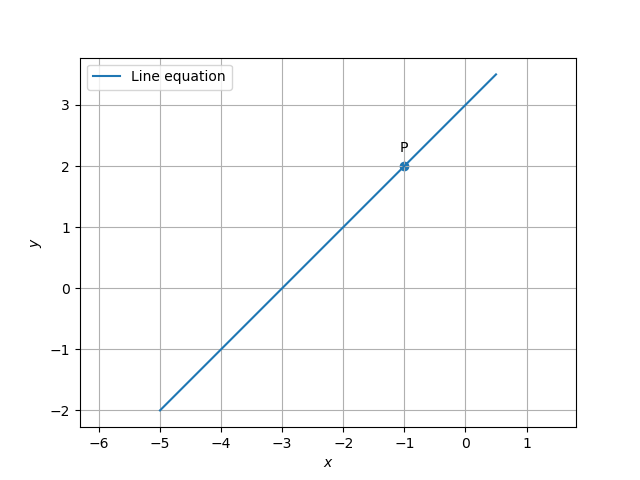
\includegraphics[width=\columnwidth]{fig.png}
\caption{}
  \label{fig:Figure}
\end{figure}
\end{document}